% ====================================================================
%+
% SECTION:
%    AGN_Microlensing.tex
%
% CHAPTER:
%    AGN.tex
%
% ELEVATOR PITCH:
%    Using AGN microlensing to measure the size and structure of
%    accretion disks. Depends on well-sampled multi-filter light curves,
%    and a large sample of detected strongly-lensed AGN.
%
% COMMENTS:
%
%
% BUGS:
%
%
% AUTHORS:
%    Timo Anguita (@tanguita)
%-
% ====================================================================

\section{AGN Size and Structure with Microlensing}
\def\secname{\chpname:microlensing}\label{sec:\secname}

\credit{tanguita}

% This individual section will need to describe the particular
% discoveries and measurements that are being targeted in this section's
% science case. It will be helpful to think of a ``science case" as a
% ``science project" that the authors {\it actually plan to do}. Then,
% the sections can follow the tried and tested format of an observing
% proposal: a brief description of the investigation, with references,
% followed by a technical feasibility piece. This latter part will need
% to be quantified using the MAF framework, via a set of metrics that
% need to be computed for any given observing strategy to quantify its
% impact on the described science case. Ideally, these metrics would be
% combined in a well-motivated figure of merit. The section can conclude
% with a discussion of any risks that have been identified, and how
% these could be mitigated.

% A short preamble goes here. What's the context for this science
% project? Where does it fit in the big picture?

Microlensing due to stars projected on top of individual
gravitationally-lensed quasar images produces additional magnification.
Using the fact that the Einstein radii of stars in lensing galaxies
closely match the scales of different emission regions in
high-redshift AGNs (micro-arcseconds), analyzing microlensing induced
flux variations statistically on individual systems allows us to
measure ``sizes'' of AGN regions.

Assuming a thermal profile for accretion disks, sizes in different emission 
wavelengths will be probed and as such, placing constraints on the slope of this 
thermal profile. Given the sheer number of lensed systems that LSST is expected 
to discover ($\sim8000$), this will allow us to stack systems for better 
constraints and hopefully determine the {\it luminosity and redshift evolution 
of the disk size and profile.} Due to the typical relative velocities of lenses, 
microlenses, observers (Earth) and source AGN, the microlensing variation 
timescales are between months to a few decades.

% --------------------------------------------------------------------

\subsection{Target measurements and discoveries}
\label{sec:\secname:targets}

% Describe the discoveries and measurements you want to make.

% Now, describe their response to the observing strategy. Qualitatively,
% how will the science project be affected by the observing schedule and
% conditions? In broad terms, how would we expect the observing strategy
% to be optimized for this science?

Analysis of microlensing induced variability will allow the measurement of 
accretion disk sizes $R_\lambda$ and their thermal profile slope $\alpha$. This 
needs to be done per system discovered. Assuming $\sim$1000 lensed quasars with 
high quality light curves (i.e. that allow time delay measurements, see 
\autoref{sec:lenstimedelays}), a relationship between size, thermal profile 
slope, black hole mass and accretion disk luminosity will likely be derived.

How precisely are we going to be able to measure these parameters for a given 
survey strategy? This is not a simple question to answer due to the significant 
degeneracies that plague the phenomenon. This is what our MAF metric will 
quantify. Before we design this, we need to predict and statistically quantify 
the degeneracies and sensitivities.

% \new{Our goal is to understand the population of AGN accretion disk sizes
% and profiles. We anticipate doing this via a hierarchical model where
% these properties are related to each other in some way, perhaps via
% power law scaling relations. A very simple version of this is the following...
% \newline\newline
% So, our targets are the parameters $a$ and $b$, that describe this
% simple population. How well will we be able to measure these, for a
% given survey strategy? This is what our MAF metric will quantify.
% Before we design this, we can predict the likely sensitivities of this
% measurement.}

The quasar microlensing optical depth is $\sim1$, so every lensed quasar should 
be affected by microlensing at any given point in time to a different extent. 
Note, however, that the larger the apparent magnification, the more stringent are
the constraints on the geometric information that can be obtained of the source. 
\citet{MosqueraandKochanek2011} studied the expected microlensing 
timescales for all known lensed quasars at the time. They found that the median 
Einstein crossing time scales, which can statistically be interpreted as the 
time between high magnification events, in the observed $I$-band, is of the order 
of $\sim20$~yr (with a distribution between 10 and 40~yr). Additionally, the source 
crossing time (duration of a high magnification event) is $\sim7.3$~months (with 
a distribution tail up to 3~yr). This basically means that out of all the lensed 
quasar {\em images} (microlensing between images is completely uncorrelated) 
about half of them will be quiescent during the 10~yr baseline of LSST. However, 
since the typical number of lensed images is either two or four, this means 
that, statistically, in every system, one (for doubles) or two (for quads) high 
magnification events should be observed in 10~yr of LSST monitoring. 

Note that, the important cadence parameter is the source crossing time. Ideally, 
high magnification events would need to be as uniformly sampled as possible. The 
$\sim 7.3$ months crossing time is the median for the observed $i$-band, but this time 
would be significantly shorter for bluer bands: for a thermal profile with slope 
$\alpha: R_\lambda \propto \lambda^\alpha$ implies source crossing time $t_{\rm 
s} \propto \lambda^{1/\alpha} \rightarrow t_u=t_i \times (\lambda_{\rm u} / 
\lambda_{\rm i})^{1/\alpha}$. For a Shakura-Sunyaev slope of $\alpha=0.75$ this 
would correspond to $\sim 7.3 \times (3600/8140)^{4/3}$ months which is $\approx 2.5$ 
months in the $u$-band.

In terms of the cadence, at least three evenly sampled data points per band 
within two to three months would be preferred to be able to map the constraining 
high magnification event, and these would hopefully be uniformly spaced.
Additionally, LSST can trigger imaging of high-magnification events with dedicated
facilities to enhance these constraints. More frequent sampling (e.g., in the DDFs)
would increase such constraints significantly. However, since lensed quasars are not
that common, this smaller area would mean that only a modest number ($<100$)
of suitable systems will be monitored in the DDFs.

Regarding the season length, the ``months'' timescale of high
magnification events very likely means that we can/will miss high
magnification events in the season gaps, at least in the bluer bands.

``Show stopper'': observations spread on timescales larger than 3 months.
This would likely miss the high magnification events. In those cases
we could perhaps consider close consecutive photometric bands as
equivalent accretion disk regions, however this would mean weaker
constraints on the thermal profile.

{\bf Caveats:} The above estimates correspond to those obtained by 
\citet{MosqueraandKochanek2011} for all \emph{currently} known lensed quasars. 
It is important to take into consideration that the timescales directly depend 
on the projected velocities of the three-plane system: the redshifts of the lens 
and source as well as their respective peculiar velocites along the CMB dipole 
velocity in the direction towards the lensing galaxies (observer's peculiar 
velocity). Therefore, every new system will have a different timescale. 
Furthermore, the discussion above is centered on high magnification events. Even 
though these produce the most valuable information, low magnification events or 
\emph{no} magnification events can set constraints on the structure of high 
redshift AGN as well as the lensing galaxies (e.g. \citealt{gilmerino2005}). 
Finally, long timescale high accuracy multiband data as will be delivered by 
LSST have never been obtained to date for any lensed system. Coupling this fact 
to a factor $\sim$10 increase on the number of lensed quasars known, LSST will 
enable of totally new and unprecedented perspectives for microlensing studies.
%
% Important Note: all this science needs to be done on lensed quasars
% with measured or very short time delays to remove the intrinsic
% variability signal, which might significantly reduce the sample.

{\bf Microlensing Aided Reverberation Mapping:} Given that microlensing mostly 
affects continuum emission rather than BELR emission, microlensing can enable 
the disentangling of the BELR emission plus the continuum emission in single 
photometric bands, allowing the use of single broad band PRM measurements 
\citep{SluseandTewes2014}. As with the two-band PRM method discussed above, the 
denser (and the longer) the sampling, the more accurate are the constraints that 
can be obtained for the time delays. This method allows constraining both the 
accretion disk structure as explained above and the BELR. The only additional 
requirement is one spectroscopic observation to constrain the ``macro'' 
magnification ratios from narrow emission lines.
% --------------------------------------------------------------------

\subsection{Metrics}
\label{sec:\secname:metrics}

%Quantifying the response via MAF metrics: definition of the metrics,
%and any derived overall figure of merit.

Metrics for these section need to be defined by using simulated light curves 
that take into account the several parameters that come into play in quasar 
microlensing. These include: the time gap between visits in the same band, 
projected CMB velocity, simulated peculiar velocities and redshifts of lenses 
and sources as well as ``macro'' lens model parameters (i.e., surface mass 
density and shear projected on top of lensed quasar images). Two metrics are 
currently in consideration:

High Magnification Events recovery metric: This metric will measure the number of high magnification events recovered/missed considering the cadence and season length in every LSST band and as the precision of the brightness measurement.

Accretion disk size and slope metric: This metric will do a full analysis of the ``pure'' microlensing light curves to recover these two physical AGN parameters. The figure of merit would be the accuracy of the measurement.

Since microlensing signal can only be obtained after time delays between images 
have been measured, both metrics need close interaction with time delay 
measurements. As such, the ``Time Delays Challenges'' (see
\autoref{sec:lenstimedelays}) will include complete microlensing signal 
simulations which also take into account the aforementioned parameters. Note
that given 
the dependence on individual filter cadence and season length as well as 
projected CMB velocities, every region on the sky needs to be considered
independently. Time Delay Challenge submissions will thus include recovered
``pure'' microlensing 
light curves in addition to measured time-delays. By doing the reverse
procedure, i.e. using these ``pure'' microlensing light curves to statistically
re obtain the input accretion disk sizes and thermal slopes, we will be able to
quantitatively measure the accuracy of the intrinsic accretion disk parameter
estimations for a given survey strategy.



....

% microlensing - convolve microlensing timescales for QSOs we already know
% about. how many of the high magnification events do we get? How bright?
% @tanguita

% --------------------------------------------------------------------

\subsection{OpSim Analysis}
\label{sec:\secname:analysis}

Much like the cosmology with lensed quasar time delays, we expect a strong
dependence of both proposed metrics with night-to-night cadence, uniformity and
season length. Maximizing these will maximize the likelihood of recovering high
magnification events, which in turn will provide the most stringent constraints
on
accretion disk structure. As mentioned above, since shorter wavelengths show
faster and stronger magnification events, in an ideal scenario, bluer bands would have
tighter night-to-night cadence.

\begin{center}
	\begin{figure}
		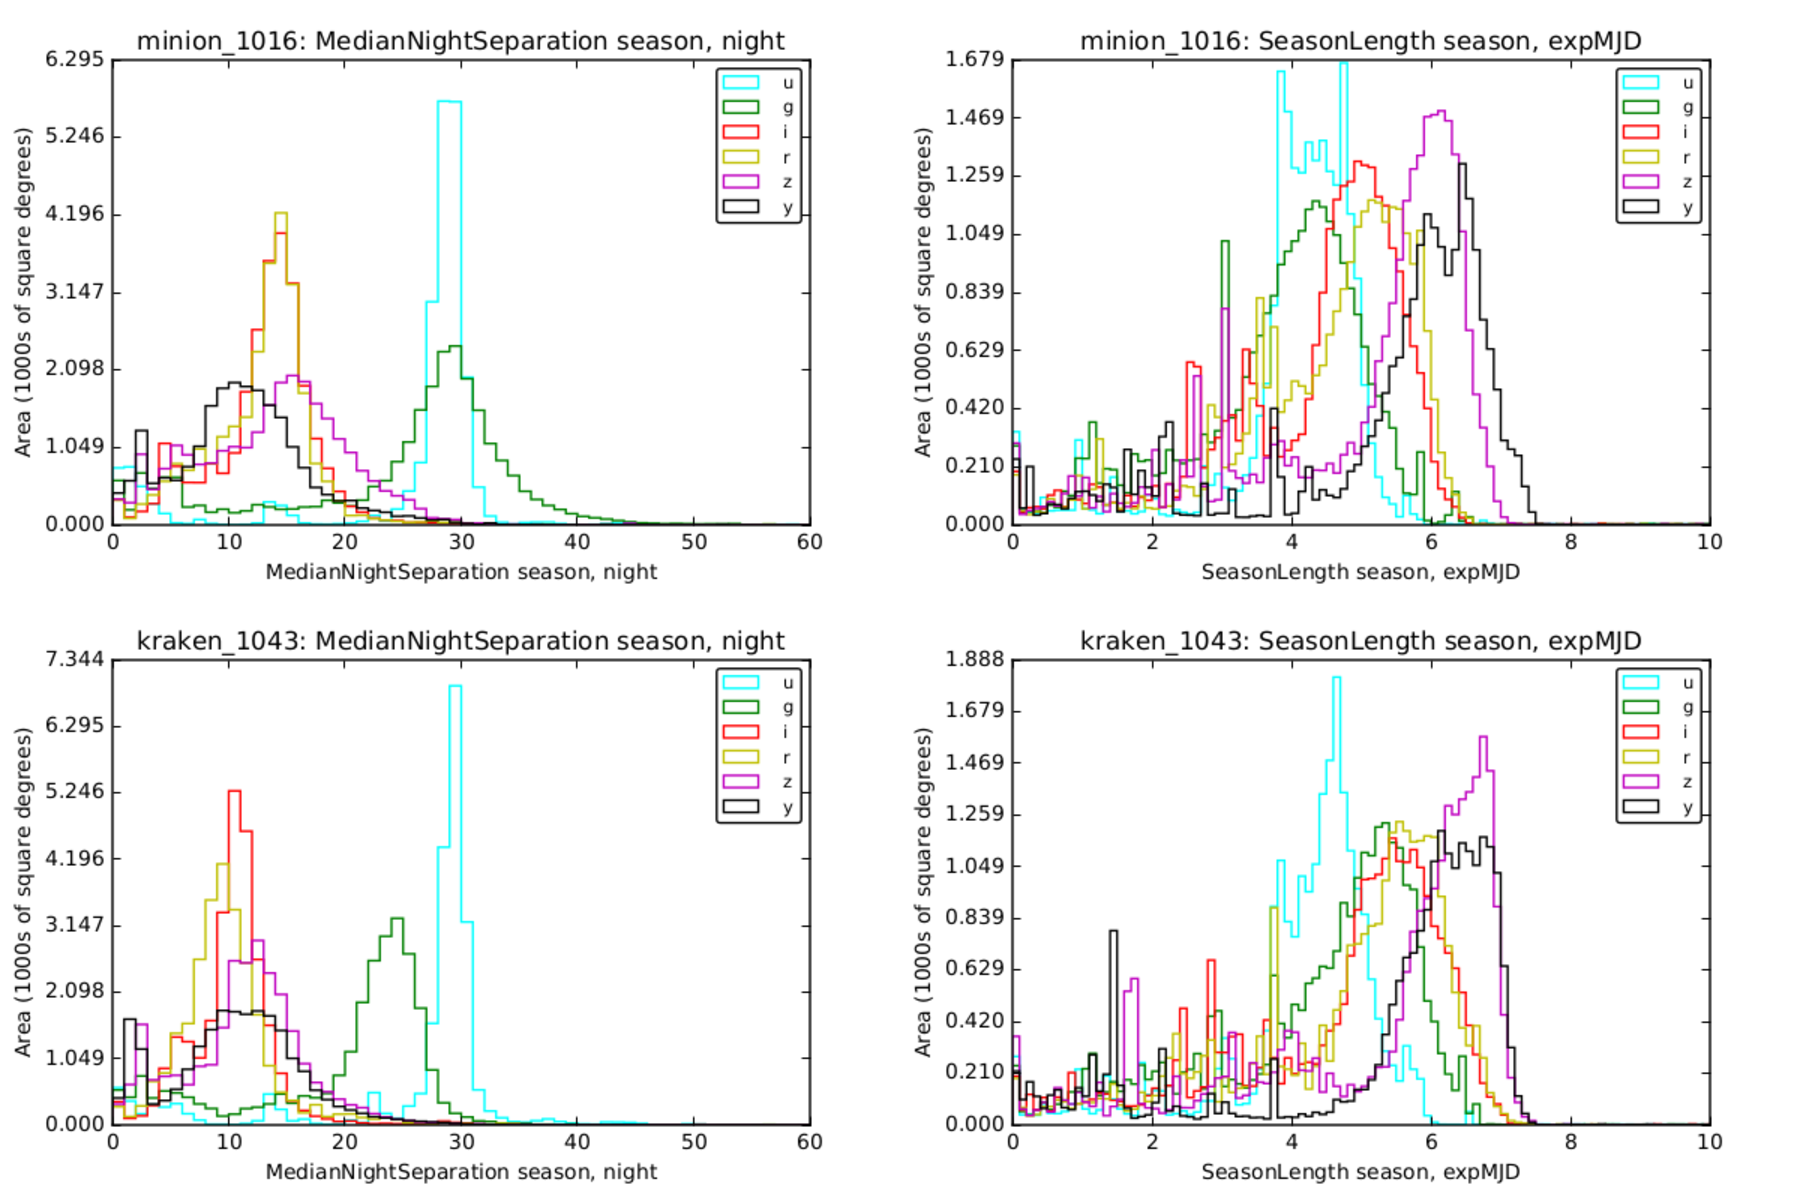
\includegraphics[width=\textwidth]{figs/agn/NightSep_seasonLength.pdf}
		\caption{Median Night Separation in days (left) and median season length in months (right) for all bands in the current ``Baseline Cadence'' (\opsimdbref{db:baseCadence}, top) and ``No Visit Pairs''	(\opsimdbref{db:NoVisitPairs}, bottom) opsim outputs.}
		\label{microfig}
	\end{figure}
\end{center}

As shown in figure \ref{microfig}, it seems there is a slightly better prospect
for the AGN structure with microlensing science case using the ``No Visit Pairs'' observing
strategy in comparison to the baseline strategy due to the smaller inter-night
gaps and longer season lengths in the g band. In both cases the night-to-night
cadence in the longer wavebands are compatible with the detection of most
microlensing events. On the other hand, in the u and g bands in both survey strategies it might compromise the results. Furthermore, in all LSST bands the spread in the night-to-night cadence (uniformity) and season length will likely dominate the uncertainties.


% --------------------------------------------------------------------

\subsection{Discussion}
\label{sec:\secname:discussion}

%Discussion: what risks have been identified? What suggestions could be
%made to improve this science project's figure of merit, and mitigate
%the identified risks?


% ====================================================================

\navigationbar
